%Este trabalho está licenciado sob a Licença Atribuição-CompartilhaIgual 4.0 Internacional Creative Commons. Para visualizar uma cópia desta licença, visite http://creativecommons.org/licenses/by-sa/4.0/deed.pt_BR ou mande uma carta para Creative Commons, PO Box 1866, Mountain View, CA 94042, USA.

\chapter{Produto misto}\label{cap_prodmisto}
\thispagestyle{fancy}

Ao longo deste capítulo, assumiremos trabalhar com uma base ortonormal positiva $B = (\vec{i},\vec{j},\vec{k})$.

\section{Definição e propriedades}\label{cap_prodmisto_sec_defn}

O {\bf produto misto} de três vetores $\vec{u}$, $\vec{v}$ e $\vec{w}$, nesta ordem, é definido por
\begin{equation}
  {\color{blue}[\vec{u},\vec{v},\vec{w}] := \vec{u}\land\vec{v}\cdot\vec{w}}.
\end{equation}

Em coordenadas, temos
\begin{gather}
  [\vec{u},\vec{v},\vec{w}] := \vec{u}\land\vec{v}\cdot\vec{w} \\
  = \begin{vmatrix}
    \vec{i} & \vec{j} & \vec{k} \\
    u_1 & u_2 & u_3 \\
    v_1 & v_2 & v_3
  \end{vmatrix} \cdot \vec{w} \\
  = \left(
    \begin{vmatrix}
      u_2 & u_3\\
      v_2 & v_3
    \end{vmatrix}\vec{i} -
    \begin{vmatrix}
      u_1 & u_3 \\
      v_1 & v_3
    \end{vmatrix}\vec{j}  +
    \begin{vmatrix}
      u_1 & u_2\\
      v_1 & v_2
    \end{vmatrix}\vec{k}\right)\cdot(w_1,w_2,w_3)\\
  = \begin{vmatrix}
    u_2 & u_3\\
    v_2 & v_3
  \end{vmatrix}w_1 -
  \begin{vmatrix}
    u_1 & u_3 \\
    v_1 & v_3
  \end{vmatrix}w_2
  + \begin{vmatrix}
    u_1 & u_2\\
    v_1 & v_2
  \end{vmatrix}w_3\\
  = \begin{vmatrix}
    w_1 & w_2 & w_3 \\
    u_1 & u_2 & u_3 \\
    v_1 & v_2 & v_3
  \end{vmatrix} \\
  = \begin{vmatrix}
    u_1 & u_2 & u_3 \\
    v_1 & v_2 & v_3 \\
    w_1 & w_2 & w_3 
  \end{vmatrix}
\end{gather}
Ou seja, temos
\begin{equation}
  {\color{blue}[\vec{u},\vec{v},\vec{w}] = \begin{vmatrix}
    u_1 & u_2 & u_3 \\
    v_1 & v_2 & v_3 \\
    w_1 & w_2 & w_3 
  \end{vmatrix}}
\end{equation}

\begin{ex}
  Dados os vetores $\vec{u} = (1,-1,0)$, $\vec{v} = (1,0,2)$ e $\vec{w} = (1,-1,1)$, temos
  \begin{align}
    [\vec{u},\vec{v},\vec{w}] &=
                                \begin{vmatrix}
                                  u_1 & u_2 & u_3 \\
                                  v_1 & v_2 & v_3 \\
                                  w_1 & w_2 & w_3       
                                \end{vmatrix} \\
                              &= \begin{vmatrix}
                                1 & -1 & 0 \\
                                1 & 0  & 2 \\
                                1 & -1 & 1       
                              \end{vmatrix} \\
                              &= 1
  \end{align}
\end{ex}

\subsection{Interpretação geométrica}\label{subsec:pm_ig}

Consideramos uma base positiva $(\vec{u},\vec{v},\vec{w})$, com $\vec{u}=\overrightarrow{AB}$, $\vec{v}=\overrightarrow{AD}$ e $\vec{w}=\overrightarrow{AH}$. Conforme vemos na Figura \ref{fig:pm_ig}, estes vetores determinam um paralelepípedo.

\begin{figure}[H]
  \centering
  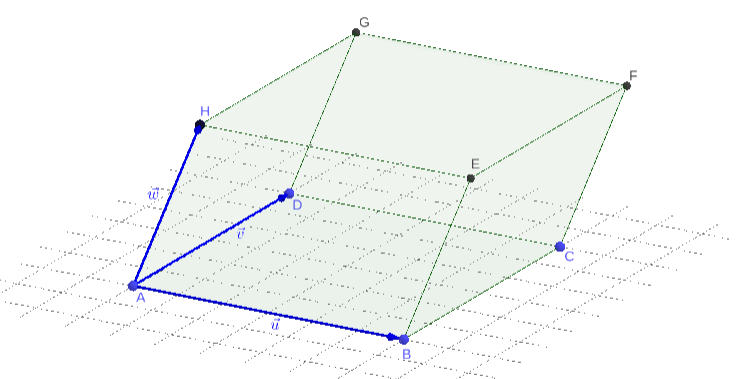
\includegraphics[width=0.8\textwidth]{cap_prodmisto/dados/fig_pm_ig/fig_pm_ig}
  \caption{Interpretação geométrica do produto misto.}
  \label{fig:pm_ig}
\end{figure}

A base do paralelepípedo é o paralelogramo $ABCD$ de área $|\vec{u}\land\vec{v}|$. Assim sendo, o \emph{volume do paralelepípedo} é
\begin{equation}\label{eq:pm_aux1}
  V = |\vec{u}\land\vec{v}|\cdot h,
\end{equation}
onde $h$ é a altura do prisma. Por sua vez,
\begin{align}
  h &= \left|\proj_{\vec{u}\land\vec{v}}\vec{w}\right| \\
    &= \left|\frac{\vec{w}\cdot(\vec{u}\land\vec{v})}{|\vec{u}\land\vec{v}|^2}\vec{u}\land\vec{v}\right|\\
    &= \frac{\left|\vec{w}\cdot(\vec{u}\land\vec{v})\right|}{|\vec{u}\land\vec{v}|^2}|\vec{u}\land\vec{v}|\\
    &= \frac{\left|\vec{w}\cdot(\vec{u}\land\vec{v})\right|}{|\vec{u}\land\vec{v}|} 
\end{align}
Logo, retornando a \eqref{eq:pm_aux1}, obtemos
\begin{align}
  V &= |\vec{u}\land\vec{v}|\cdot h\\
    &= |\vec{u}\land\vec{v}|\cdot\frac{\left|\vec{w}\cdot(\vec{u}\land\vec{v})\right|}{|\vec{u}\land\vec{v}|} \\
    &= \left|\vec{w}\cdot(\vec{u}\land\vec{v})\right|\\
    &= \left|\vec{u}\land\vec{v}\cdot\vec{w}\right|.
\end{align}
Ou seja, o \emph{volume do paralelípedo} formado pelos vetores $\vec{u}$, $\vec{v}$ e $\vec{w}$ é igual a norma do produto misto destes vetores, i.e.
\begin{equation}\label{eq:pm_vp}
  {\color{blue}V = |[\vec{u},\vec{v},\vec{w}]|}.
\end{equation}

\begin{ex}
  Vamos calcular o volume do paralelepípedo determinado pelos vetores $\vec{u}=(1,1,0)$, $\vec{v}=(-1,2,0)$ e $\vec{w}=(0,1,1)$. De \eqref{eq:pm_vp}, temos
  \begin{gather}
    V = |[\vec{u},\vec{v},\vec{w}]| \\
    = \left|
      \begin{vmatrix}
        1 & 1 & 0 \\
        -1 & 2 & 0 \\
        0 & 1 & 1
      \end{vmatrix}
    \right| \\
    = |3| = 3.
  \end{gather}
\end{ex}

\subsection{Propriedades}

Valem as seguintes propriedades:
\begin{enumerate}[a)]
\item {\color{blue}$[\vec{u},\vec{v},\vec{w}] = -[\vec{v},\vec{u},\vec{w}]$}

  {\it Demonstração}. De fato, quando permutamos duas linhas em uma matriz, seu determinante troca de sinal.
  
\item {\color{blue}$[\vec{u},\vec{v},\vec{w}] = -[\vec{u},\vec{w},\vec{v}]$}

  {\it Demonstração.} Mesmo argumento da letra a).
  
\item {\color{blue}$[\vec{u},\vec{v},\vec{w}] = [\vec{w},\vec{u},\vec{v}] = [\vec{v},\vec{w},\vec{u}]$}

  {\it Demonstração.} De fato, cada caso acima corresponde a duas consecutivas permutações de linha na matriz associada ao produto misto.
  
\item {\color{blue}$[\vec{u},\vec{v},\vec{w}] = \vec{u}\land\vec{v}\cdot\vec{w} = \vec{u}\cdot\vec{v}\land\vec{w}$}

  {\it Demonstração.} Isto segue de c), i.e.
  \begin{align}
    [\vec{u},\vec{v},\vec{w}] &= [\vec{v},\vec{w},\vec{u}] \\
    \vec{u}\land\vec{v}\cdot\vec{w} &= \vec{v}\land\vec{w}\cdot\vec{u}\\
                              &= \vec{u}\cdot\vec{v}\land\vec{w}.
  \end{align}
  
\item {\color{blue}$[\alpha\vec{u},\vec{v},\vec{w}] = [\vec{u},\alpha\vec{v},\vec{w}]=[\vec{u},\vec{v},\alpha\vec{w}] = \alpha[\vec{u},\vec{v},\vec{w}]$}

  {\it Determinação.} De fato, ao multiplicarmos uma linha de uma matriz por um escalar $\alpha$, seu determinante fica multiplicado por $\alpha$.
  
\item {\color{blue}$[\vec{u}+\vec{z},\vec{v},\vec{w}] = [\vec{u},\vec{v},\vec{w}]+[\vec{z},\vec{v},\vec{w}]$}

  {\it Determinante.} Também segue da propriedade análoga do determinante de matrizes.
\end{enumerate}

\begin{ex}
  Sabendo que $[\vec{u},2\vec{w},\vec{v}] = 2$, vamos calcular $[\vec{u},\vec{v},\vec{w}]$. Do item e) acima, temos
  \begin{align}
    2 &= [\vec{u},2\vec{w},\vec{v}] \\
      &= 2[\vec{u},\vec{w},\vec{v}],
  \end{align}
  donde
  \begin{equation}
    [\vec{u},\vec{w},\vec{v}] = 1.
  \end{equation}
  Agora, do item b), temos
  \begin{equation}
    [\vec{u},\vec{w},\vec{v}] = -[\vec{u},\vec{v},\vec{w}].
  \end{equation}
  Ou seja, concluímos que $[\vec{u},\vec{v},\vec{w}] =  -1$.
\end{ex}

Também, temos as seguinte propriedades envolvendo o produto misto:
\begin{enumerate}[a)]
\item Se ${\color{blue}[\vec{u},\vec{v},\vec{w}] = 0}$, então ${\color{blue}(\vec{u},\vec{v},\vec{w})}$ \emph{não é base}.

  {\it Demonstração}. Seja $[\vec{u},\vec{v},\vec{w}]=0$, i.e. $\vec{u}\land\vec{v}\cdot\vec{w}=0$. No caso de um dos vetores serem nulos, então $(\vec{u},\vec{v},\vec{w})$ não é base. Suponhamos, então, que $\vec{u}$, $\vec{v}$ e $\vec{w}$ são vetores não nulos. Isso implica que $\vec{u}\land\vec{v}=0$ ou $(\vec{u}\land\vec{v})\perp\vec{w}$. No primeiro caso, $\vec{u}$ e $\vec{v}$ são l.d. e, portanto, $(\vec{u},\vec{v},\vec{w})$  não é base. No segundo caso, $(\vec{u}\land\vec{v})\perp\vec{w}$, temos que $\vec{w}$ é coplanar aos vetores $\vec{u}$ e $\vec{v}$, logo $(\vec{u},\vec{v},\vec{w})$ não é base.
  
\item Se ${\color{blue}[\vec{u},\vec{v},\vec{w}] > 0}$, então ${\color{blue}(\vec{u},\vec{v},\vec{w})}$ é uma \emph{base positiva}.

  {\it Demonstração.} Se $[\vec{u},\vec{v},\vec{w}] > 0$, implica que o ângulo entre $\vec{u}\land\vec{v}$ e $\vec{w}$ é agudo, o que garante que $(\vec{u},\vec{v},\vec{w})$ seja uma base positiva.
  
\item Se ${\color{blue}[\vec{u},\vec{v},\vec{w}] < 0}$, então ${\color{blue}(\vec{u},\vec{v},\vec{w})}$ é uma \emph{base negativa}.

  {\it Demonstração.} Se $[\vec{u},\vec{v},\vec{w}] < 0$, implica que o ângulo entre $\vec{u}\land\vec{v}$ e $\vec{w}$ é obtuso, o que garante que $(\vec{u},\vec{v},\vec{w})$ seja uma base negativa.
\end{enumerate}

\subsection*{Exercícios resolvidos}

\begin{exeresol}
  Calcule a área do paralelogramo determinado pelos vetores $\vec{v}=(1,0,-2)$, $\vec{w}=(1,-2,1)$ e $\vec{u}=(0,2,1)$.
\end{exeresol}
\begin{resol}
  Da Subseção \ref{subsec:pm_ig}, temos que o volume do paralelogramo é
  \begin{equation}
    V = |[\vec{u},\vec{v},\vec{w}]|,
  \end{equation}
  não importando a ordem dos vetores\footnote{A ordem dos vetores não altera o módulo do valor do produto misto.}. Assim sendo, temos
  \begin{gather}
    V = |[\vec{u},\vec{v},\vec{w}]| \\
    = \left|
      \begin{vmatrix}
        0 & 2 & 1 \\
        1 & 0 & -2 \\
        1 & -2 & 1 
      \end{vmatrix}
    \right| \\
    = |-8| = 8.
  \end{gather}
\end{resol}

\emconstrucao

\subsection*{Exercícios}

\emconstrucao